% Changing book to article will make the footers match on each page,
% rather than alternate every other.
%
% Note that the article class does not have chapters.
\documentclass[letterpaper,10pt,twoside,twocolumn,openany]{book}

% Use babel or polyglossia to automatically redefine macros for terms
% Armor Class, Level, etc...
% Default output is in English; captions are located in lib/dndstring-captions.sty.
% If no captions exist for a language, English will be used.
%1. To load a language with babel:
%	\usepackage[<lang>]{babel}
%2. To load a language with polyglossia:
%	\usepackage{polyglossia}
%	\setdefaultlanguage{<lang>}
\usepackage[english]{babel}
%usepackage[italian]{babel}
% For further options (multilanguage documents, hypenations, language environments...)
% please refer to babel/polyglossia's documentation.

\usepackage[utf8]{inputenc}
\usepackage{lipsum}
\usepackage{listings}
\usepackage{multicol}
% dnd package options 
% bg-full   : Default option. Use paper background and fancy footer.
% bg-print  : Use fancy footer but not background.
% bg-none   : No paper background and plain footer.
% justified : Use full justification for text layout instead of ragged right.
\usepackage{standalone}
\usepackage{dnd}
\usepackage{mwe}
\usepackage{afterpage}
\usepackage{adjustbox}
\usepackage{bbding}
%\usepackage{hyperref}
\usepackage{graphicx} % Required for including images
\usepackage[font=small,labelfont=bf]{caption} % Required for specifying captions to tables and figures
\usepackage{pdfpages}
\lstset{%
  basicstyle=\ttfamily,
  language=[LaTeX]{TeX},
}

% Start document
\begin{document}
%% B.tex
\documentclass{standalone}
% your preamble here
\begin{document}
% your diagram code here
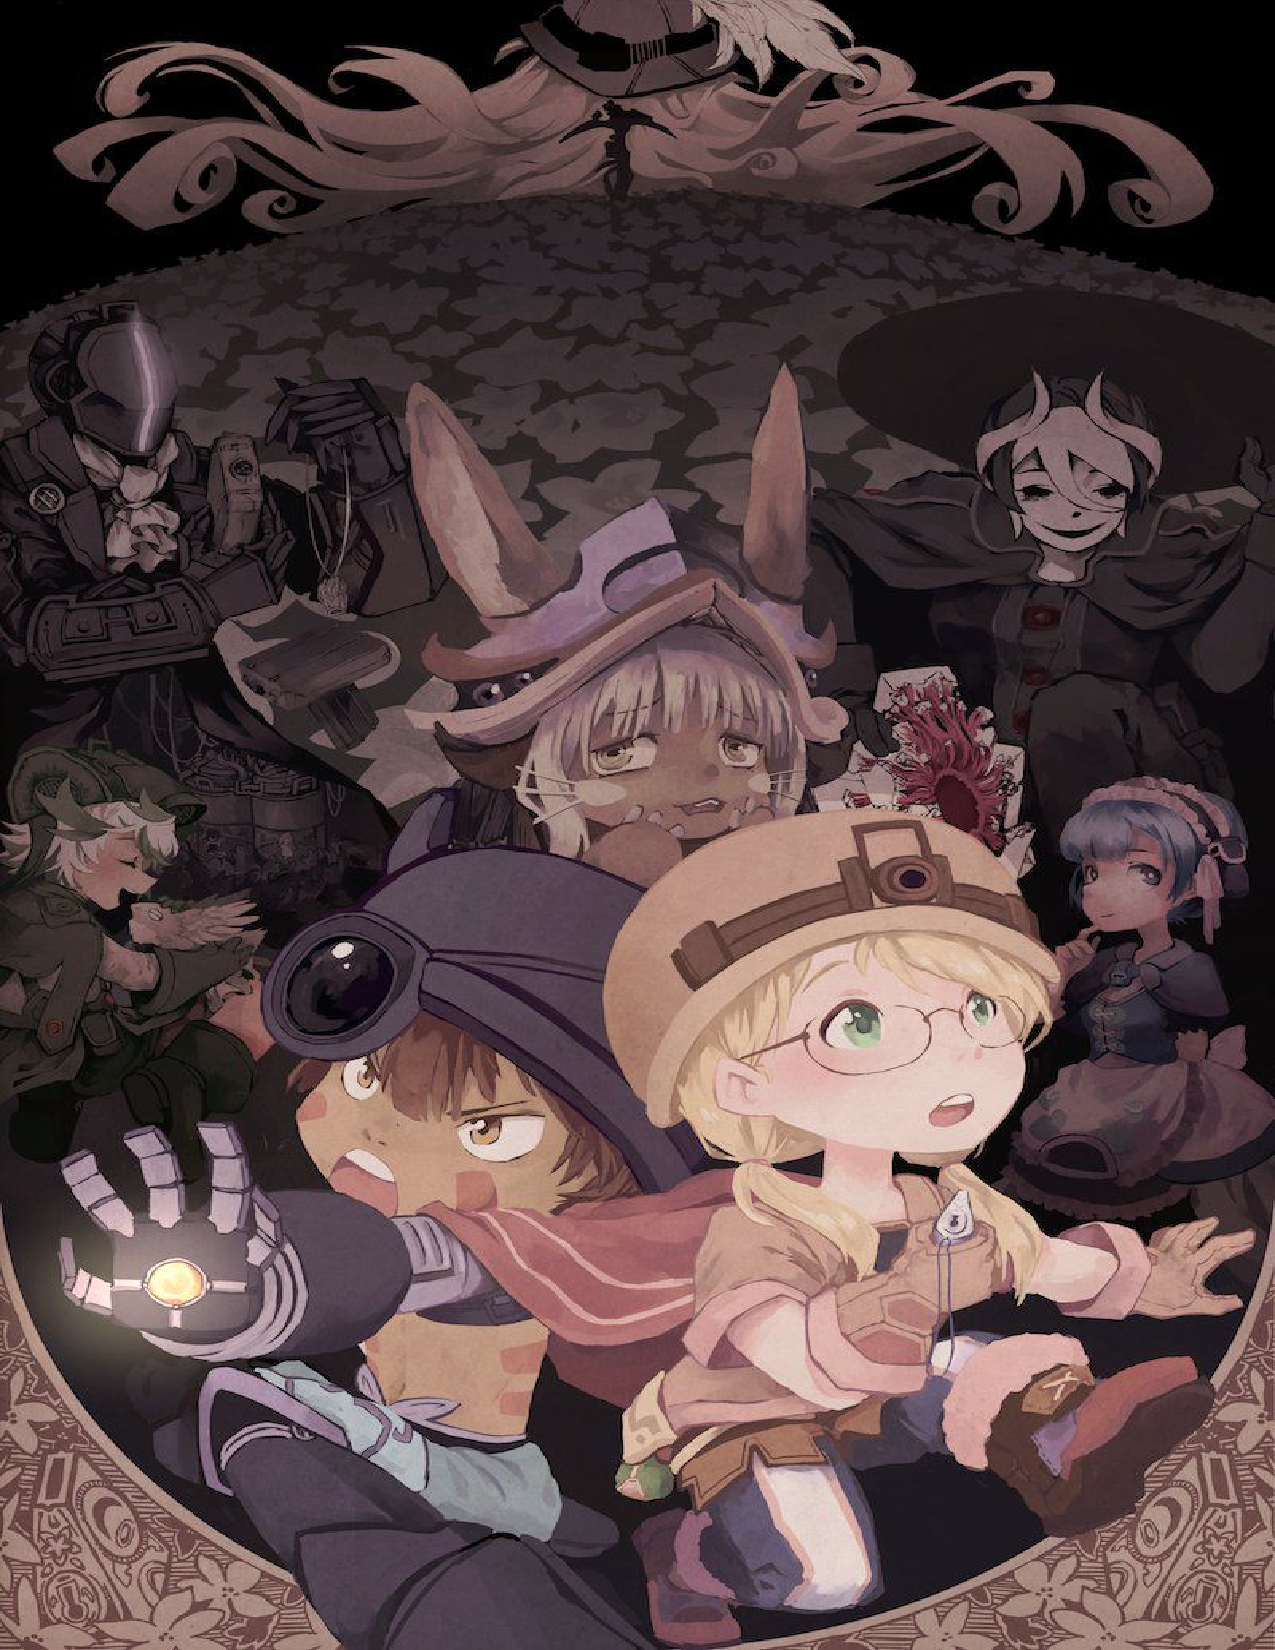
\includepdf{img/cover/cover2}
\end{document}

%%\tableofcontents

\chapter{Made in Abyss}

\section{System Rules v0.01}
This document outlines a module that extends existing systems, such as \textit{Dungeons \& Dragons} and \textit{Dungeon World}. It consists mostly of mechanics to supplement a Made in Abyss campaign.

\section{SPOILERS AHEAD!} 
Be afraid, verry afraid! The document contains extensive spoilers from both the anime and manga. If you have not caught up yet, consider avoid reading this document until you have. 

\section{Sources}
\header{Delvers \& Whistles:}
The background descriptions have been coped from the Wikia article. 

\header{Curse:}

\header{Images:}
\newline The curse's effects images are from the Anime adaption of Made in Abys.

\section{Acknowledgement}
This document would not have been possible without the help from the community. Special thanks to the the amazing work by authors on the Made in Abyss Wikia\footnote{http://madeinabyss.wikia.com/wiki/Made\_in\_Abyss\_Wiki} and the dedicated fans on the Made in Abyss subreddit. 

\subsection{Feedback!}
The module is a work-in-progress so feedback is very much appreciated! Forward them to me at microhive@gmail.com.

%\tableofcontents
%\listoffigures
%\listoftables
\chapter{Delvers}

\section{Delvers of Orth}
The champions of this story are the delvers also known as cave raiders. Their mission is to explore the abyss, retrieve its many riches, and discover its many mysteries. However, their descent is fraught with danger and unforeseen encounters, often to their untimely demise. They are considered folk heroes by the \textit{town of Orth}. The town is built around the edge of the abyss. 

\section{Background \& Motives}

Delver's motivations for delving the abyss are varied. Some are drawn to it from a competitive aspect, others for its many wonderous treasures, and others from pure curiosity about its many secrets. What they all have in common is their undying desire to brave the abyss to attain their goal.

\begin{quotebox}
"If it was between dying of old age, or of some stupid thing like a heart attack... I'd want to die exploring the great unknown, and satisfying that urge to see the endless nameless." \newline\textit{Øbserver, a blue whistle}
\end{quotebox}

\header{Whistle Illustrations}

\begin{center}
\begin{tabular}{c}
\adjustbox{trim=0 0 0 0,clip}{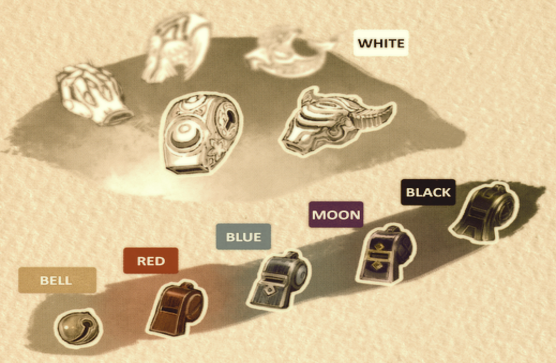
\includegraphics[width=7.5cm]{img/delvers/1.png}} \\
 \end{tabular}
\captionof{figure}{e) Descending into the 6th layer is known as the Last Dive. Curses beyond this point are severe and lethal for humans.}
\end{center}

\section{Delvers' Whistles}
All delvers (*) are equipped with a whistle. They represents their wearers social status within Orth and their expertise as delvers of the Abyss. Experienced delvers can travel further down without severe consequences. They have a better understanding of the layout and dangers of each of the layers. 

In terms of mechanics delvers' rank describe which layers is most appropriate for their level. See table 1.1.

\header{Delvers' Rank}
\begin{dndtable}[llX]
    \textbf{Title} & \textbf{Position} & \textbf{Deepest Layer}\\
    Bell whistle & Student & Surface \\
    Red whistle & Apprentice & 1st \\
    Blue whistle & Adept & 2rd \\
    Moon whistle & Teacher & 3rd \\
    Black whistle & Expert & 4th \\
    White whistle & Legendary & 5th+\footnote{See section "The Last Dive"\ref{se:thelastdive}, p. \pageref{se:thelastdive}}  \\
\end{dndtable}
\label{tab:colors}

\subsection{Bell Whistles}
Work in Progress.

\subsection{Red Whistles}
The apprentices. Red Whistles are rookie delvers who have a decent knowledge of the abyss and have descended up to the first layer on their own. It is a common rank for prepubescent kids who have studied since an early age. One obtains a red whistle and the official title of delver after they first descent to the abyss. While they're fairly knowledgeable, red whistles lack the physical fortitude to get very deep, so they're only allowed to descend up to 550 meters. Going any deeper would be treated as an accident or a rebellious behavior, and a rescue party would be sent to retrieve them. If a red whistle somehow managed to descend 1350 meters, it is treated as suicide and search parties are called off. 

\subsection{Blue Whistles}
The adepts. Blue Whistles are more experienced delvers who managed to proved themselves. They're allowed to delve up to the second layer of the abyss, so they most likely possess an acceptable fighting ability to fend off from the beasts of the forest of temptation. Typically and with the appropriate training, one attains the rank of blue whistle at the age of 15, though there are exceptions to this. 

\subsection{Moon Whistles}
The teachers. Moon Whistles are highly proficient delvers that carry an extensive knowledge of the abyss. They can delve up to the third layer safely, so their delving ability is in a completely different level to Blue Whistles. They're considered experienced enough to serve as teachers for the newer generations. 

\subsection{Black Whistles}
The experts. Black Whistles are extremely talented delvers that have mastered the delving techniques of delvers. They can reach up to the fourth layer of the abyss, which is the point in which the strains of ascension can really make one touch insanity. Black Whistles also sometimes work under white whistles as subordinates, and assist them in their expeditions. 

\subsection{White Whistles}
The legends. White Whistles are considered to be the greatest delvers of all. Their achievements have changed the world and their discoveries astonished all, turning into spectacular historical figures. They're named after their unique persona and reach a whole new level incomparable to that of other delvers. They're armed to the teeth with artifacts of the abyss, and represent a formidable force. Because of their status, any information that is officially passed by them is considered a fact, no matter how absurd.

Only a handful of delvers attain this legendary rank, and only five white whistles are known:

\header{Known White Whistles}
\begin{dndtable}[lX]
  \textbf{Name} & \textbf{Title} \\
  Lyza the Annihilator & The Lord of Annihilation \\
  Ozen the Immovable & The Immovable Sovereign \\
  Bondrewd the Novel & The Lord of Dawn \\
  Srajo the Obscure & The Lord of Mystery \\
  Wakuna & The Lord of Guidance \\
\end{dndtable}

\subsubsection{The Last Dive} \label{se:thelastdive}
White Whistle don't have any depth limit, however since the strains of ascension make it humanly impossible to survive the ascent from the 6th layer, for most of their life the 5th layer is their limit. At some point when they make the decision, a white whistle will descend to the inviolable 6th layer. Since return from this point is impossible, this descent is called the "Last Dive" and it represents the most important point of their career, delving into largely unknown territory.

\section{Equipment}
Work in Progress.
\chapter{Descending the Abyss}

\section{The Abyss}
In the middle of Orth lies the legendary abyss. It is a circular chasm that is 1 km across. It is a source of great pride and challenge, as well as worship for many of its citizens. The Abyss is fraught with dangers and is very difficult to navigate. Maps are spotty at best, and information is scarce. Most knowledge is shared from mouth to mouth. 

\begin{center}
\begin{tabular}{c}
\adjustbox{trim=0 0 0 0,clip}{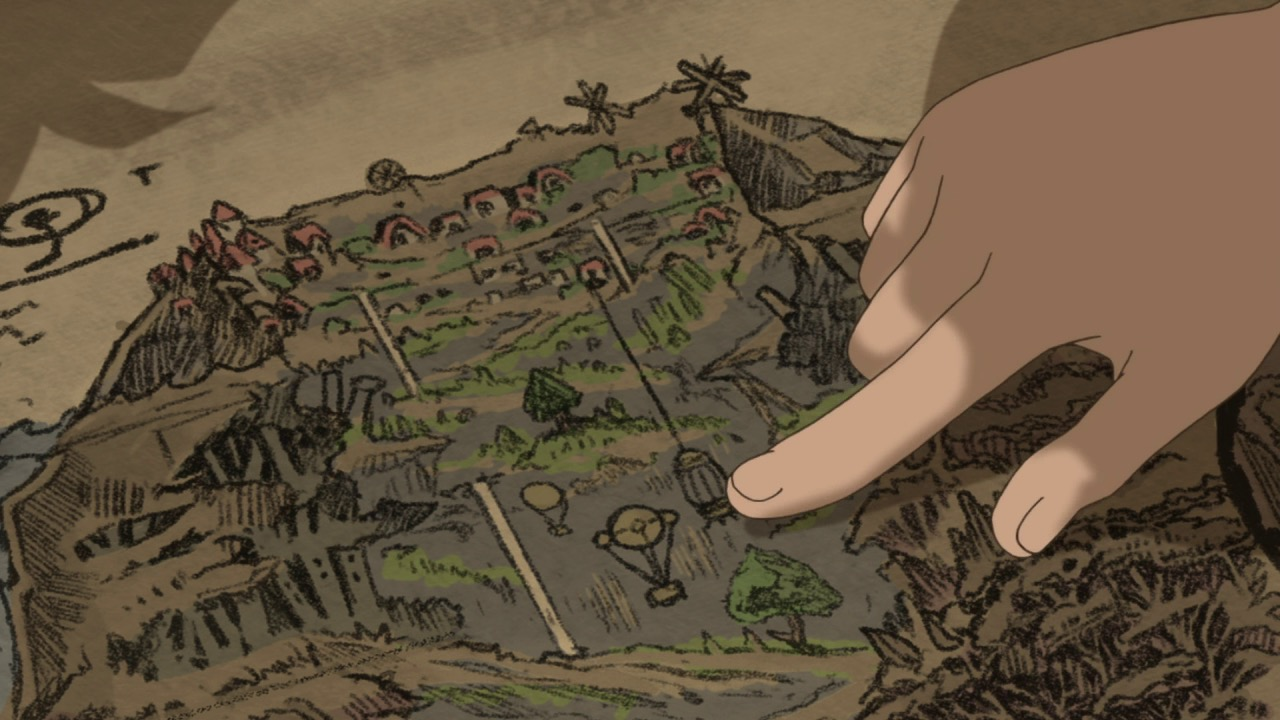
\includegraphics[width=8cm]{img/delvers/2.jpg}} \\
 \end{tabular}
\captionof{figure}{ Illustration of the village of Orth at the top, at the edge of the abyss. A delver pointing to its lower parts.}
\end{center}

\begin{table*}[t]
\header{Layers of the Abyss}
\centering
    \begin{dndtable}[clrX]
    \textbf{Layer} & \textbf{Name} & \textbf{Deepest (m)} & \textbf{Description}   \\
    Surface & Town of Orth                     & $0$     &                      \\
            1st & Edge of the Abyss                    & $1350$     &                      \\
            2nd & Forest of Temptation                 & $2600$     &                   \\
            3rd & Great Fault                          & $7000$     &                   \\
            4th & The Goblet of Giants                 & $12000$    &                   \\
            5th & Sea of Corpses                       & $13000$    &                  \\
            6th & The Capital of the Unreturned        & $15500$    &                  \\
            7th & The Final Maelstrom                  & ?            &                  \\
            8th &The Deepest Point                     & $>20000$   &                                \\
  \end{dndtable}
  \caption{Layers of the Abyss}
\end{table*}

\section{Dungeoneering}

Makes sense to tell the DM that any dungeon they can find would fit the abyss. A giant mushroom, a dungeon in an upside down windmill, underwater dungeon exploration. What is on the edge of the abyss's many layers? Sprinkle many different monsters. Take inspiration from here!

\section{Creatures of the Abyss}

Delvers diving into the abyss find themselves in a totally different ecosystem compared to the surface world. However, they will also discover themselves no longer on the top of the food chain. Delvers who have encountered creatures have categorized them depending on their danger level. The following table describes their levels. 

\header{Creature Classes}\label{tab:CreatureClasses}
\begin{dndtable}[lXc]
    \textbf{Class}  & \textbf{Rating} & \textbf{D\&D CR} \\
    Harmless    & \FiveStarOpen & 0\\
    Minor   & \FiveStar & 1\\
    Caution & \FiveStar \FiveStar & 2\\
    Serious & \FiveStar \FiveStar \FiveStar & 3-5\\
    Lethal  & \FiveStar \FiveStar \FiveStar \FiveStar & 6-9\\
    Irrational  & \FiveStar \FiveStar \FiveStar \FiveStar \FiveStar & 10-12\\
    Extraordinary   & \FiveStar \FiveStar \FiveStar \FiveStar \FiveStar \FiveStar & 13-15\\
    Unprecedented   & \FiveStar \FiveStar \FiveStar \FiveStar \FiveStar \FiveStar \FiveStar & 16+\\
\end{dndtable}

%\header{Creature Illustration}
%\begin{center}
%\begin{tabular}{c}
%\adjustbox{trim=0 0 0 %0,clip}{\includegraphics[width=8cm]{img/descending/151169500795%197.jpg}} \\
% \end{tabular}
%\captionof{figure}{ Drawing illustrations of creatures from the %lower depths of the abyss. Drawn by the white whistle, Lyza the %Annihilator. }
%\end{center}

Not only will delvers meet monstrous creatures, they will also find themselves in conflict with other delvers from foreign countries, looking to cash in on the abyss's treasures. These are considered hostile and should be disposed off. 

\subsection{Monster Manual \& Other Resources}
The opinion of the author is that the monster manual should be used sparingly, if ever. The argument is that this is a world that relies on exploration, as such, players need to feel a sense of wonder, awe, and dread, whenever they observe new settings and creatures. To achieve this effect, consider using the monster resources found at the \textbf{Monster A Day subreddit r/monsteraday/}\footnote{https://www.reddit.com/r/monsteraday/}. Each creature is descripted using 5 edition D\&D stat blocks with art work.

Choose creatures that fit the theme of each layer. When describing an encounter's difficulty, describe its visible features, and if applicable, allow players to consult their lexicon on creatures of the abyss. Use the creature class naming scheme during play to make players uneasy\ref{tab:CreatureClasses}.

\section{Artifacts}
Artifacts or relics are classified and cataloged according to their power. All artifacts have limited number of uses, often indicated by the strange writings on them. The most powerful artifacts that a white whistle can use are second grade artifacts. Greater artifacts are considered very important to national security and can be found deep within the abyss. 

\begin{quotebox}
	The discovery of a Greater Artifact is a huge ordeal. Experts and White whistles are tasked with their retrieval. These trips are perilous, as such, often come at the great cost of many lives. Greater artifacts are not cataloged, or only partially, to keep them secret from other nations, thus keeping an edge in the power struggle.
\end{quotebox}

\header{Artifact Classes}
\begin{dndtable}[lX]
  \textbf{Classes} & \textbf{Description} \\
  Special Grade Artifact            &  \\
  First Grade Artifact            &  \\
  Second Grade Artifact            &  \\
  Third Grade Artifact            &  \\
  Fourth Grade Artifact            &  \\
\end{dndtable}

\newpage

\begin{figure}[ht]
  \afterpage{%
    \noindent
    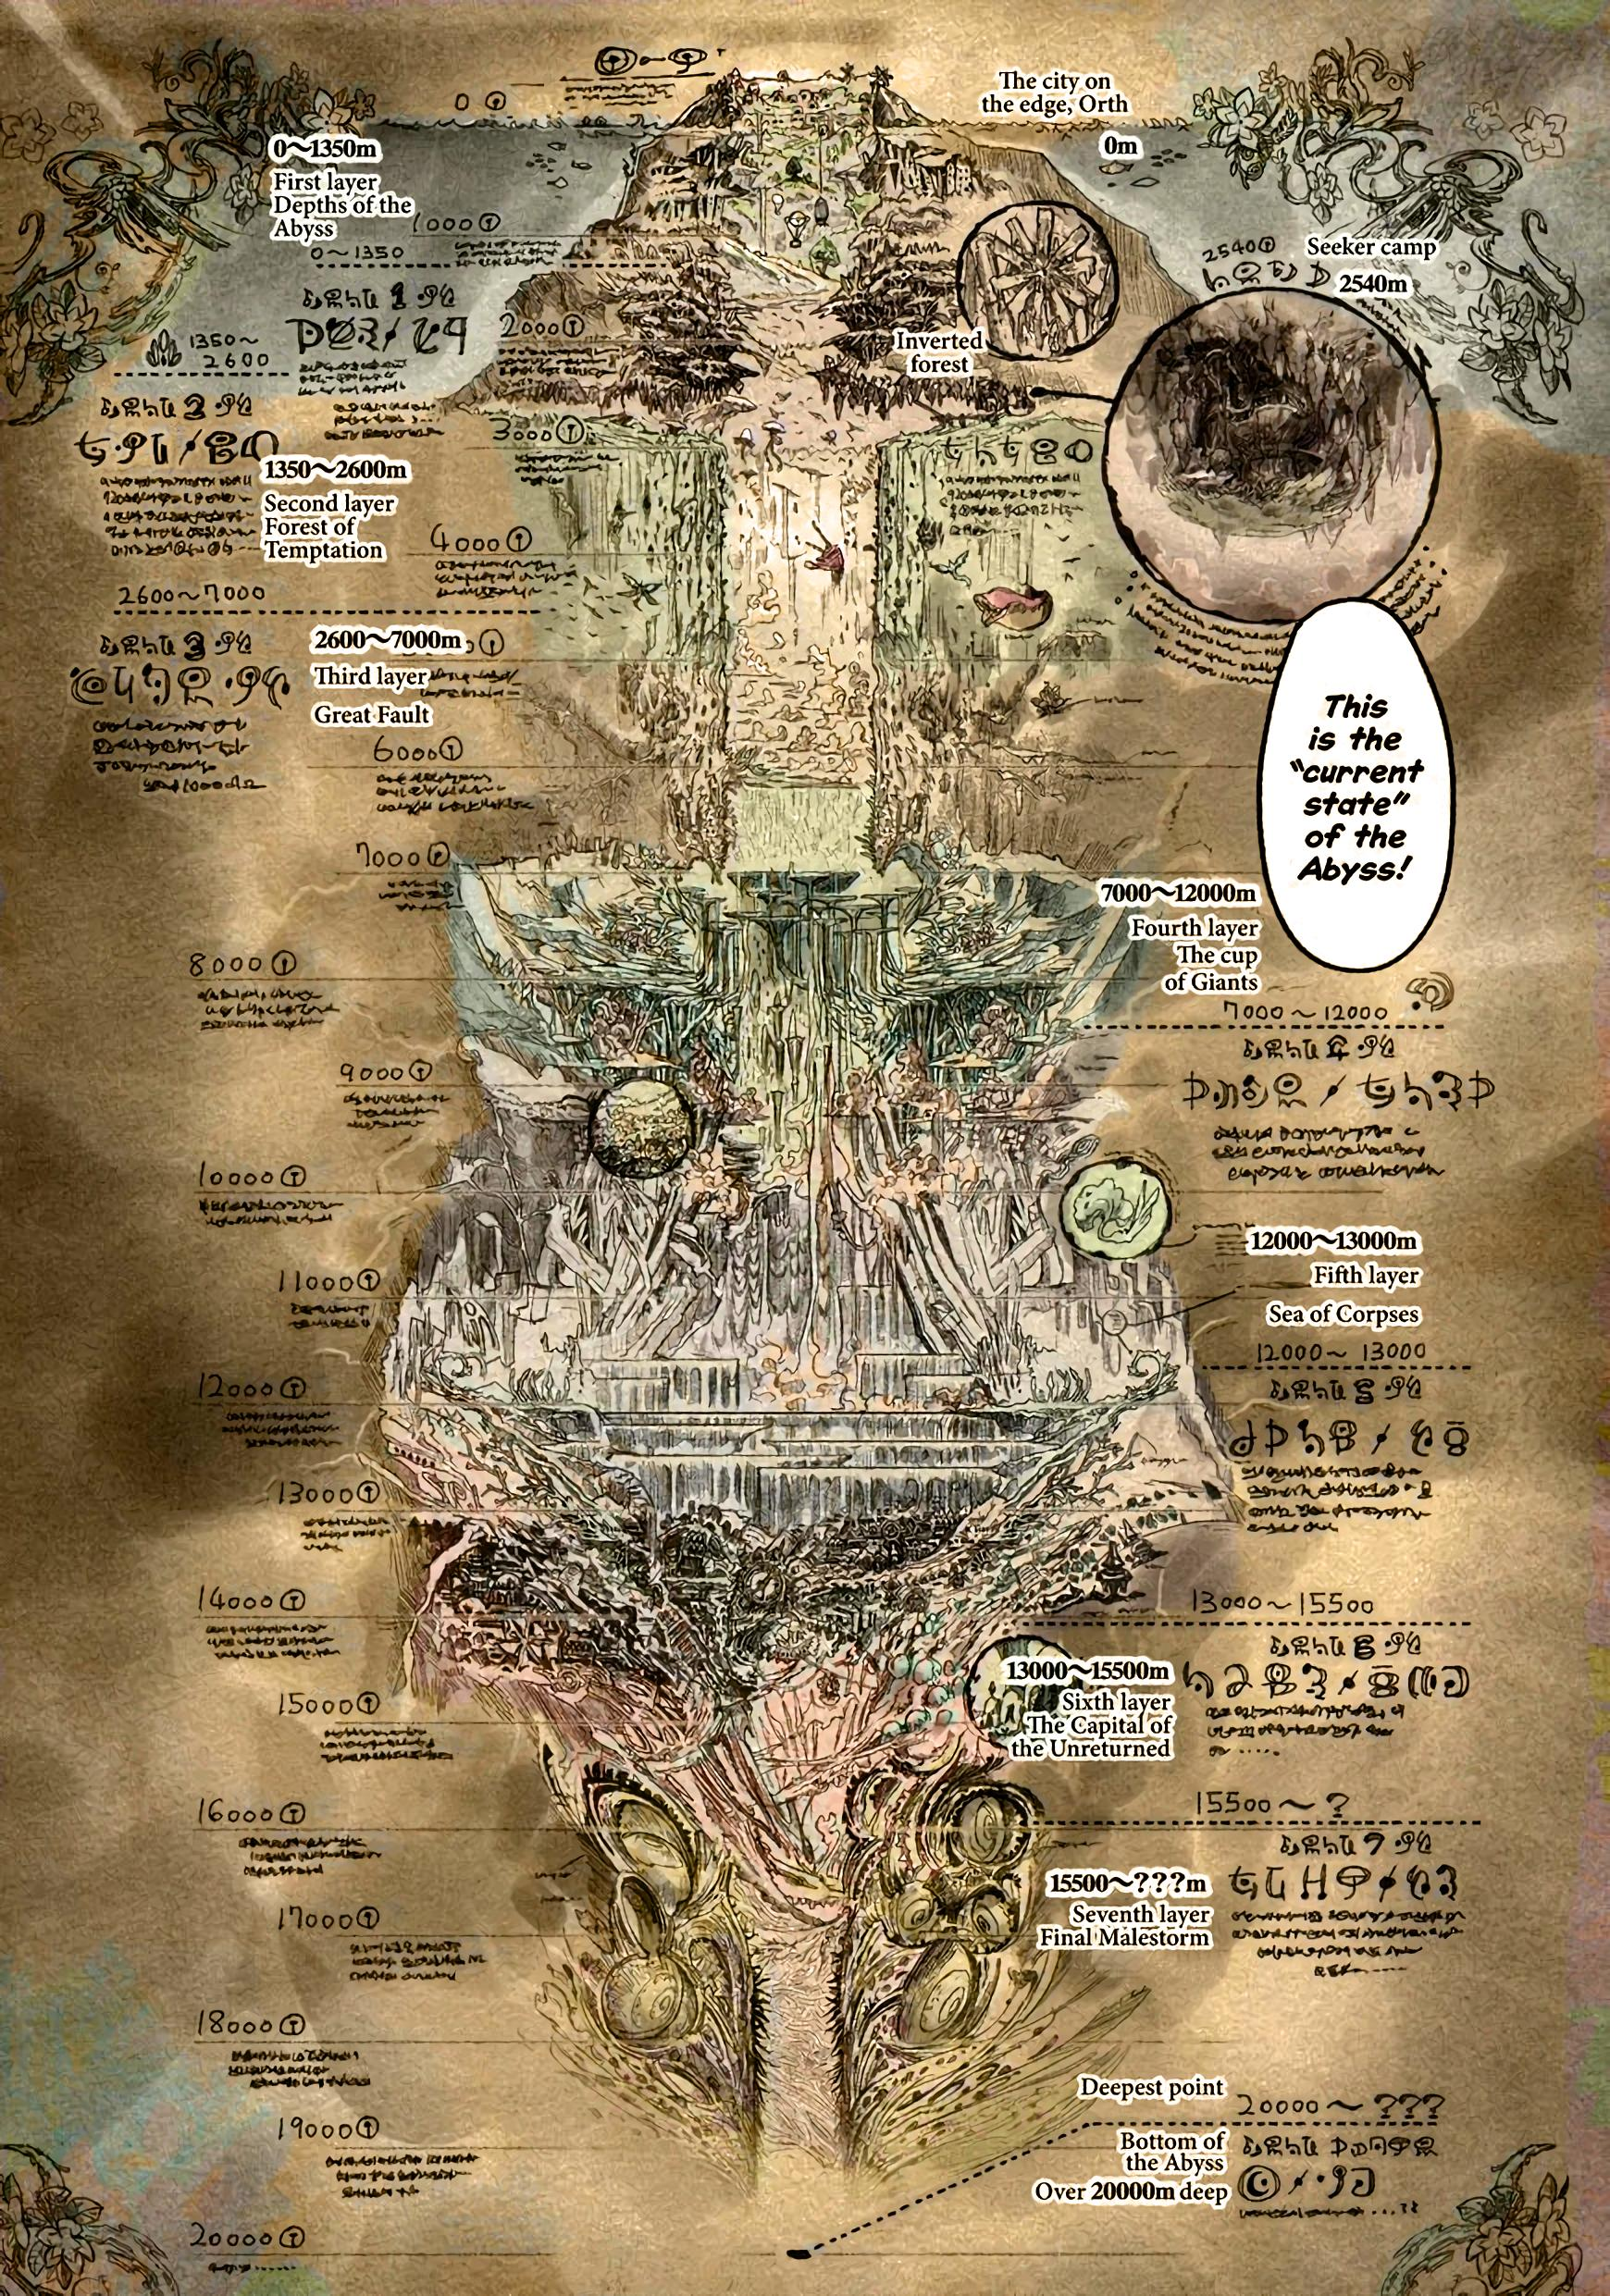
\includegraphics[width=\textwidth,height=.999\textheight]{img/descending/1506982818380.jpg}% Large image
    \clearpage
  }
  %\caption{Known map of the Abyss}
\end{figure}
\chapter{Curse of the Abyss}

\section{Ascending the Abyss}
The abyss harbors a mysterious phenomenon known as the Curse of the Abyss. It manifests when delvers attempt to ascent the abyss. This curse makes ascending a daunting affair, resulting in exhaustion and distress, even for the most seasoned delver. The deeper you go ascend from the more severe the curse's effect will be. The illustrations show some of the curse's effects.

\subsection{Exhaustion Points}
{All delvers start their descent with 0 exhaustion points out of a maximum of 3.}

\subsection{Roll for Exhaustion (2d6)}
{Whenever a delver attempts to ascend a layer of the abyss they must make a (2d6) exhaustion check to determine how many exhaustion points they gain. On a 10 or higher, they gain (+0) exhaustion points, 9 to 7 they gain (+1) point of exhaustion, and on a 6 or lower they gain (+2) points of exhaustion. \newline Should a delver find themselves ascending from beyond their recommended layer they will take (-2) penalty to their roll.}

\subsection{Exhaustion Recovery}
{A delver can recover from this state by taking a long rest. A delver can subtract 1 exhaustion point for each long rest. A delver that reaches the city of Orth can recover all of their exhaustion points after a short rest.}

\subsection{Exhaustion Consequences}
{Should a delver's exhaustion point reach 3, the partial effects of a layer's curse will apply. An affected delver succumbs to their exhaustion - and is unable to move on their own nor perform any actions. They are in a constant state of drifting in and out of consciousness. \newline In the case that their exhaustion point should exceed 3 the effects of the curse will have its full effect on the delver. In the worst case scenario depending on the description of the curse the delver dies.}

%\begin{figure*}%[ht!]
\begin{center}
\begin{tabular}{cc}
\adjustbox{trim={.25\width} 0 {0.25\width} 0,clip}{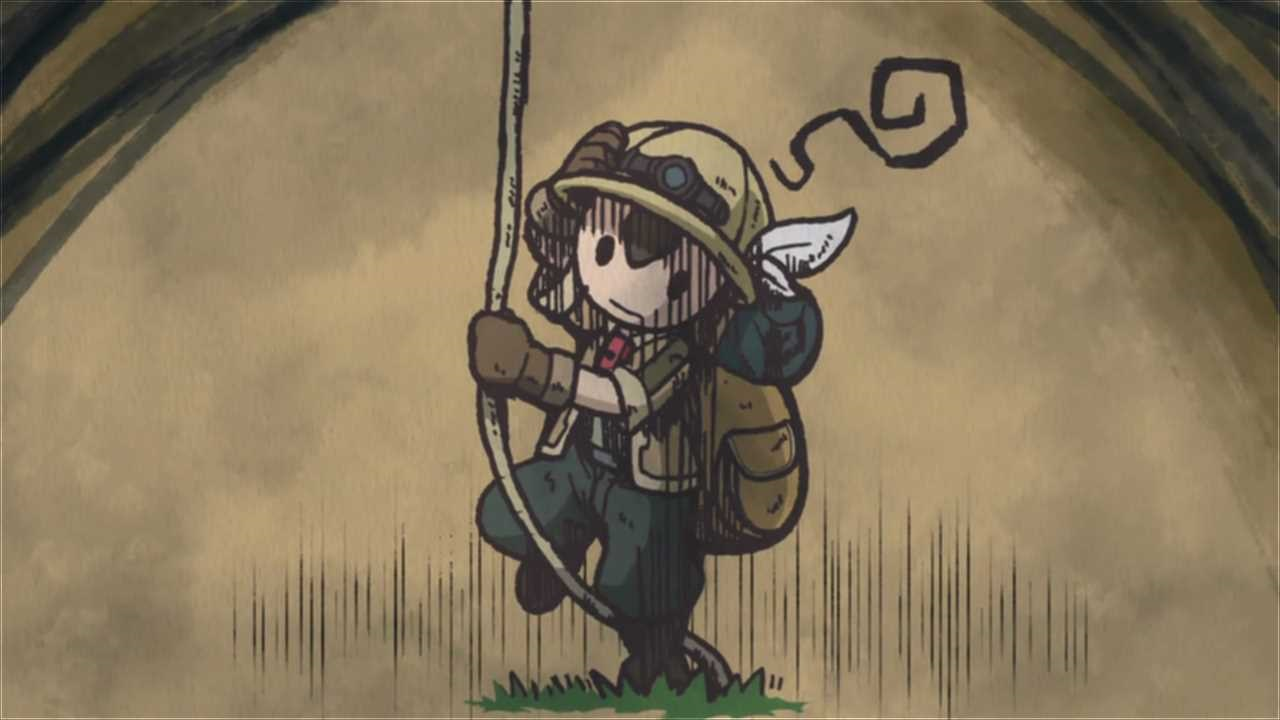
\includegraphics[width=7.3cm]{img/curses/1.png}} &
\adjustbox{trim={.25\width} 0 {0.25\width} 0,clip}{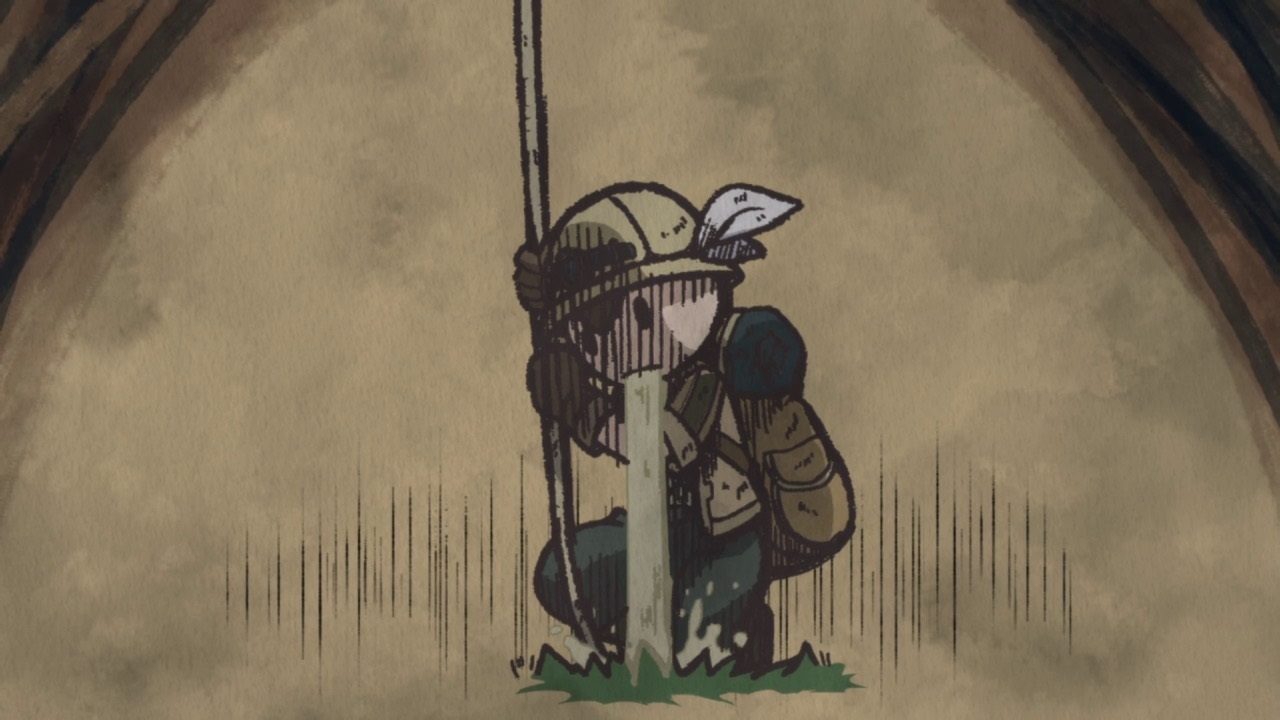
\includegraphics[width=7.3cm]{img/curses/2.png}} \\
 a) & b)\\
 \end{tabular}
\captionof{figure}{a) b) It is common for delvers who ascend from the 3rd to 1st layers to experience nausea, motion sickness, puking, and confusion.}
\end{center}
\begin{center}
\begin{tabular}{cc}
\adjustbox{trim={.25\width} 0 {0.25\width} 0,clip}{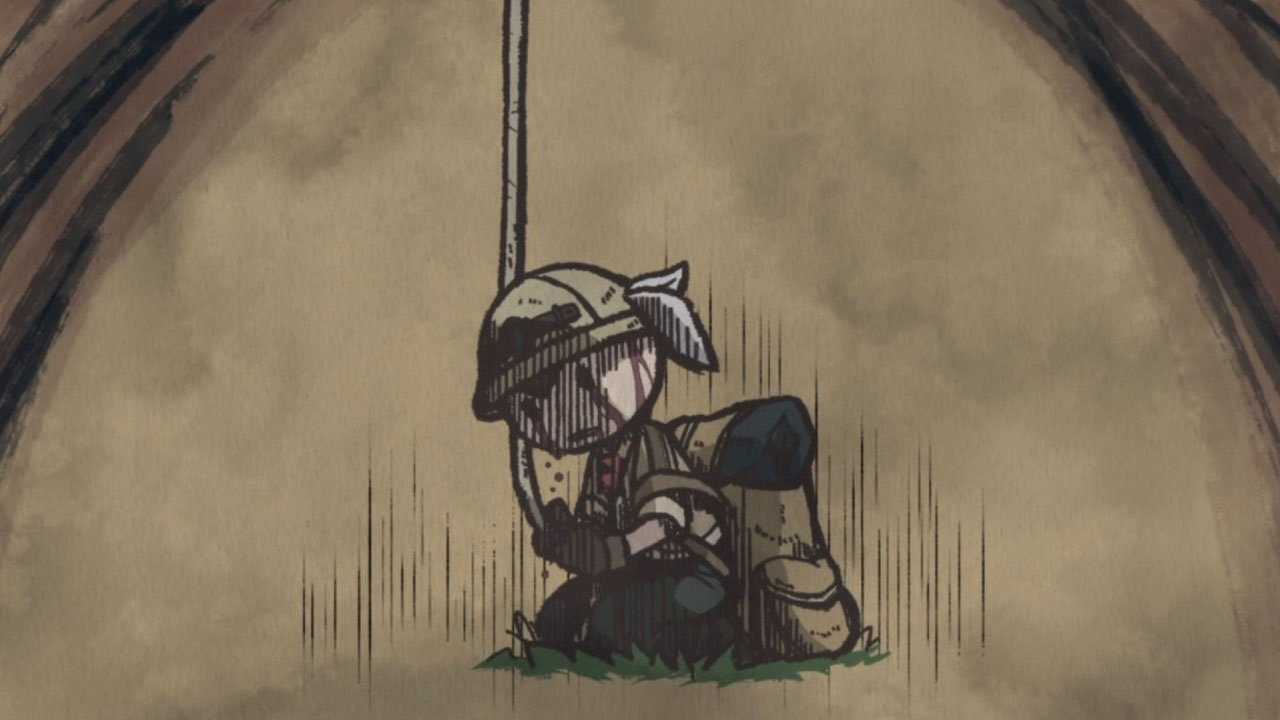
\includegraphics[width=7.3cm]{img/curses/4.png}} &
\adjustbox{trim={.25\width} 0 {0.25\width} 0,clip}{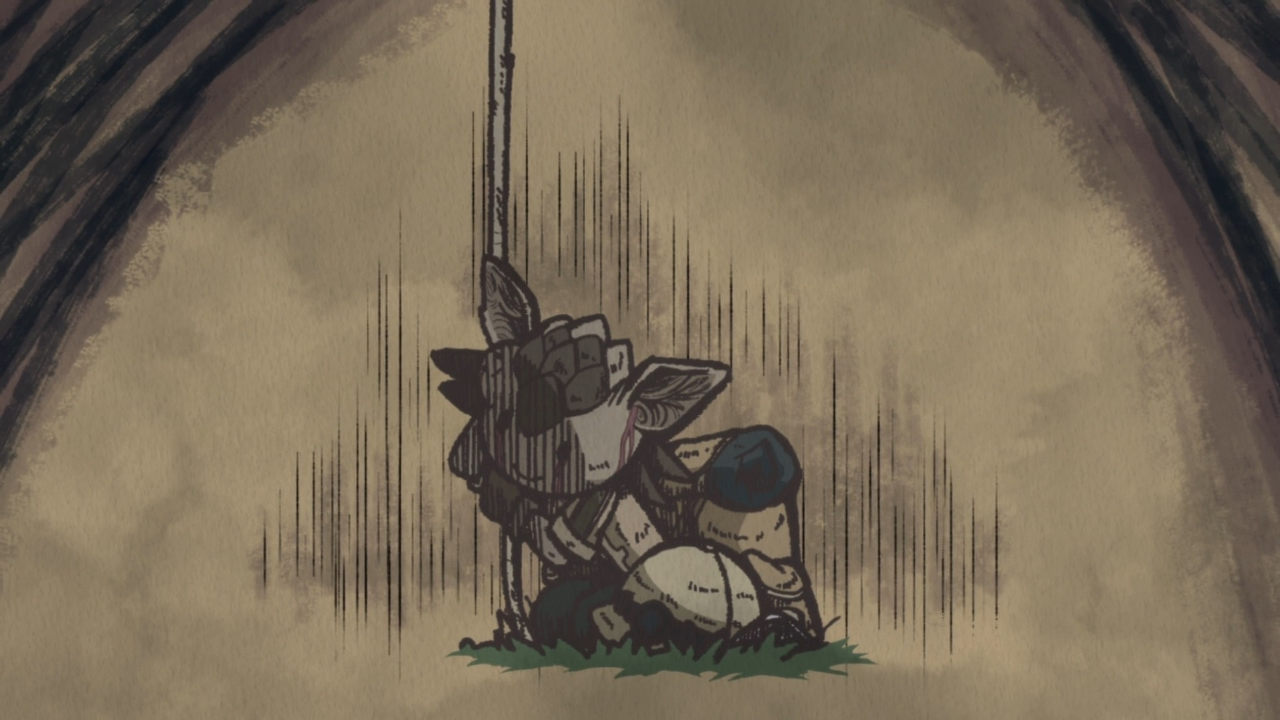
\includegraphics[width=7.3cm]{img/curses/5.png}} \\
 c) & d)\\
 \end{tabular}
\captionof{figure}{c) Delvers attempting to ascend from the 4th layer are exposed to severe hemorrhaging from all orifices. 5th layer results in intense pain and confusion resulting in self harm. d) 6th layer may result in loss of humanity. These curses can be deadly.}
\end{center}
\begin{center}
\begin{tabular}{c}
\adjustbox{trim={.1\width} 0 {0.1\width} {1cm},clip}{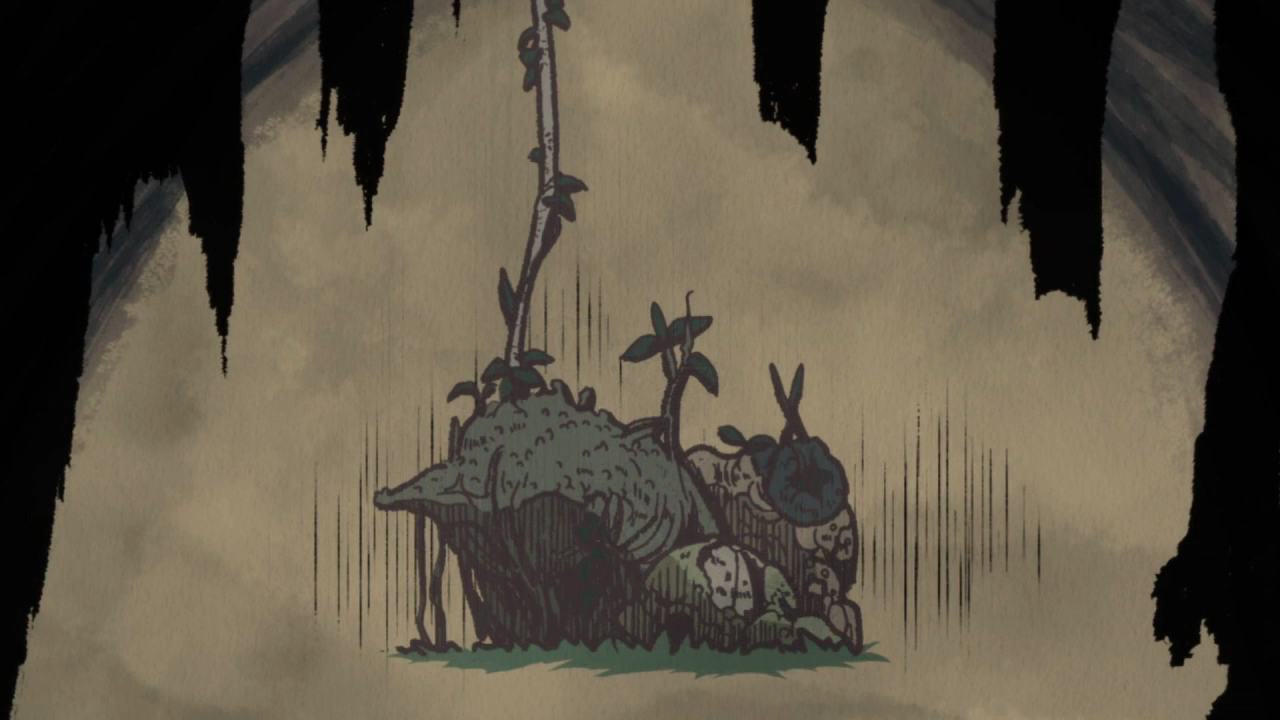
\includegraphics[width=9.5cm]{img/curses/6.png}} \\
 e)\\
 \end{tabular}
\captionof{figure}{e) Descending into the 6th layer is known as the Last Dive. Curses beyond this point are severe and lethal for humans.}
\end{center}
%\end{figure*}

\section{Humanity}

You start with 10. The effects of a lack of humanity are complex and multi-faceted. Every failure you experience will reduce your humanity.

Whenever a person 

\subtitlesection{Healthy, 20}
{You are a well-adjusted, normal human being.}

\subtitlesection{Shaken, 19-16}
{You are worldly and have experienced hardship in your life, though you aren’t necessarily less moral or worse of a person because of that.}

\subtitlesection{Shaken, 15-13}
{Your life experiences have left you callous and shrewd, distant from others from the tragedies you have lived through. Still not necessarily bad, however.}

\subtitlesection{Shaken, 13-10}
{Actual physical changes occur at this threshold, as the Abyss Curse changes one due to lack of Humanity. Small physical things, like needing to look through lenses to not get headaches, fingernails falling out and not regrowing, unnatural shortness despite genetics, lack of pigment in or persistently dry skin are all symptoms of this. No mental changes, still.}

\subtitlesection{Shaken, 10-8}
{Marked mental and physical changes occur. One’s own sense of sight, smell and spatial awareness are enhanced. People exhibit clearly inhuman features at this stage: tar-black irises, extreme paleness, animal-like behaviour, a very loose grasp of morality, abnormal musculature, inability to be socially acceptable, and severe alterations of personality are all symptoms of this stage. Most White-Whistles sit in this range.}

\subtitlesection{Shaken, 7-5}
{Treading an extremely fine line between human and monster, one’s physical abilities are once again increased, though at the detriment of their sanity and biology. A total inability to understand ethics, personal space, human rights or even basic dignity. Bones harden and become harder to break, though warp and shape themselves in ways that make uncanny changes to one’s body. One can only get to this point by repeated exposure to the Curse at the 5th layer or below, or the constant abuse of certain relics. While intelligence and willpower doesn’t suffer, victims at this stage often become unnaturally fixated on one goal at a time, and will single-mindedly pursue it even to their death.}

\subtitlesection{Shaken, 4-2}
{Total loss of what makes one a human being. Most basic animals sit here. Ranging in mental ability from pack animals to slugs.}

\subtitlesection{Shaken, 1-0}
{Inanimate objects, and things with only the most basic functions. Sponges, fungi, jellyfish, plants all make up this category.}


\chapter{Playing the Game}

\adjustbox{trim={.2\width} 0 {0.2\width} 0,clip}{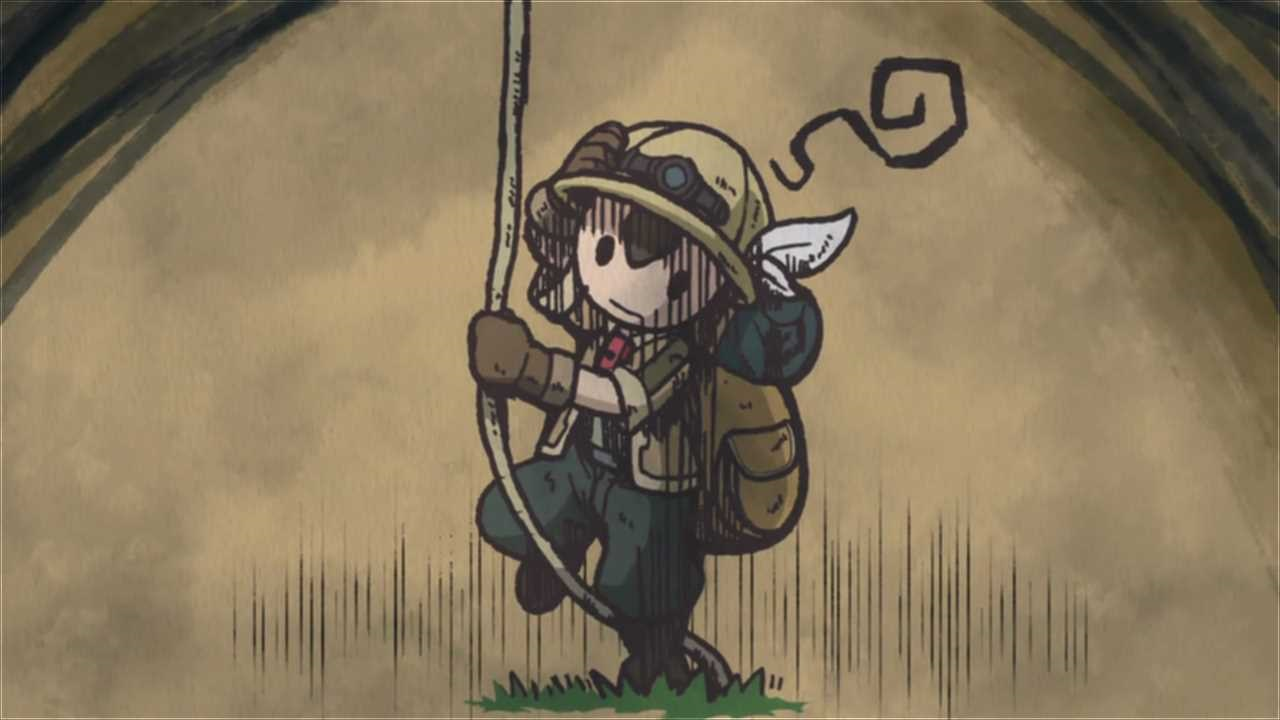
\includegraphics[width=8cm]{img/curses/1.png}}

\section{Setting up the Game}

The world of Made in Abyss is a fantastic world, however, it is not clear how you would go about adventuring in it. 

\subsection{Missions}
The world is a brutal place, and everyone will eventually be claimed by the abyss. Do you have what it takes to conquer the abyss? Are you willing to make the necessary sacrifices to survive? Only time will tell.

The following section describes scenarios you may attempt to run for shorter settings.

%Depending on how you want to pay the game, you can pick from a selection of missions form the table below. It 
\end{document}